\begin{figure}%
  \def\frac{0.24}
  \rotatebox{90}{\hspace{2em}\color{blue}{\tiny Fetch Reach}}%
  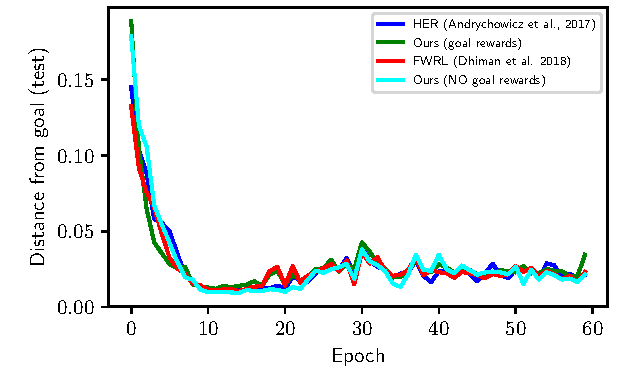
\includegraphics[width=\frac\columnwidth]{media/res/6efc1de-path_reward_low_thresh_chosen-FetchReachPR-v1-dqst/epoch-test/ag_g_dist.pdf}%
  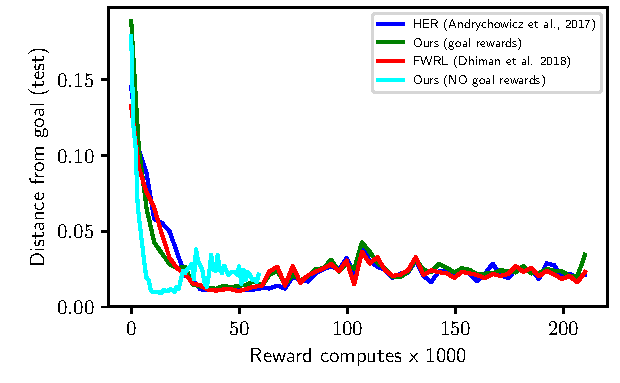
\includegraphics[width=\frac\columnwidth]{media/res/6efc1de-path_reward_low_thresh_chosen-FetchReachPR-v1-dqst/reward_computes-test/ag_g_dist.pdf}%
  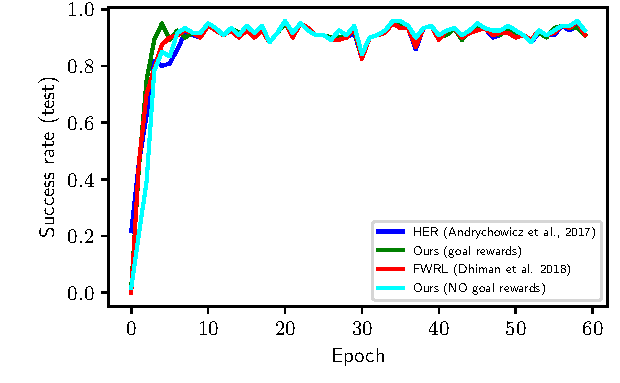
\includegraphics[width=\frac\columnwidth]{media/res/6efc1de-path_reward_low_thresh_chosen-FetchReachPR-v1-dqst/epoch-test/success_rate.pdf}%
  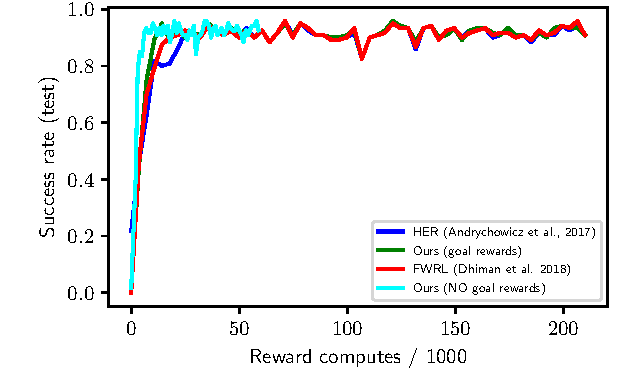
\includegraphics[width=\frac\columnwidth]{media/res/6efc1de-path_reward_low_thresh_chosen-FetchReachPR-v1-dqst/reward_computes-test/success_rate.pdf}\\
  \rotatebox{90}{\hspace{2em}\color{blue}{\tiny Fetch Push}}%
  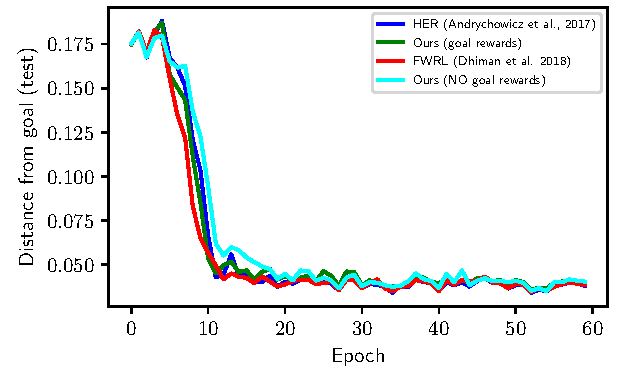
\includegraphics[width=\frac\columnwidth]{media/res/6efc1de-path_reward_low_thresh_chosen-FetchPushPR-v1-dqst/epoch-test/ag_g_dist.pdf}%
  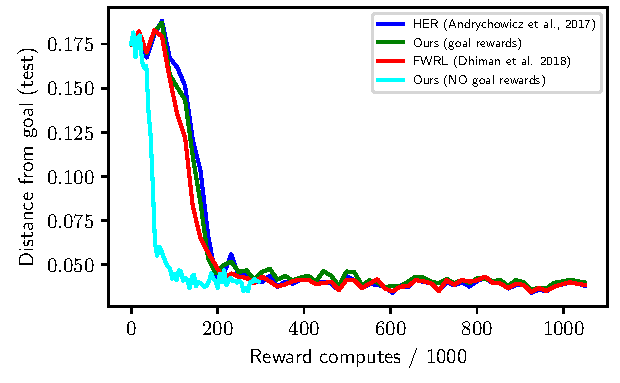
\includegraphics[width=\frac\columnwidth]{media/res/6efc1de-path_reward_low_thresh_chosen-FetchPushPR-v1-dqst/reward_computes-test/ag_g_dist.pdf}%
  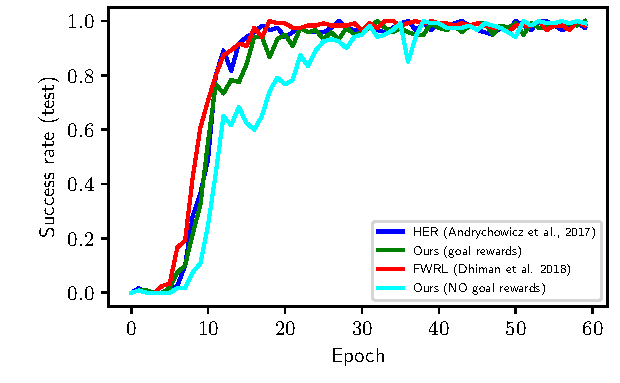
\includegraphics[width=\frac\columnwidth]{media/res/6efc1de-path_reward_low_thresh_chosen-FetchPushPR-v1-dqst/epoch-test/success_rate.pdf}%
  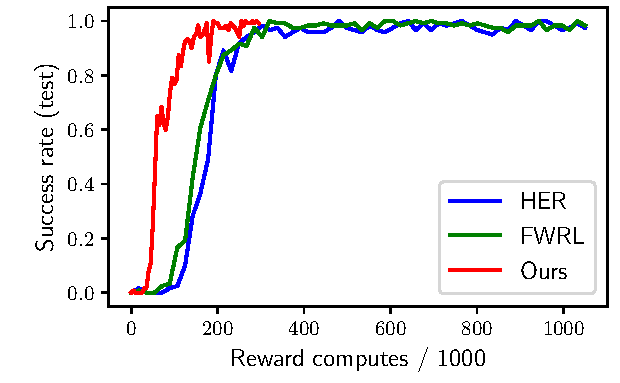
\includegraphics[width=\frac\columnwidth]{media/res/6efc1de-path_reward_low_thresh_chosen-FetchPushPR-v1-dqst/reward_computes-test/success_rate.pdf}\\
  \rotatebox{90}{{\tiny\hspace{1em} \color{blue}{Fetch Pick And Place}}}%
  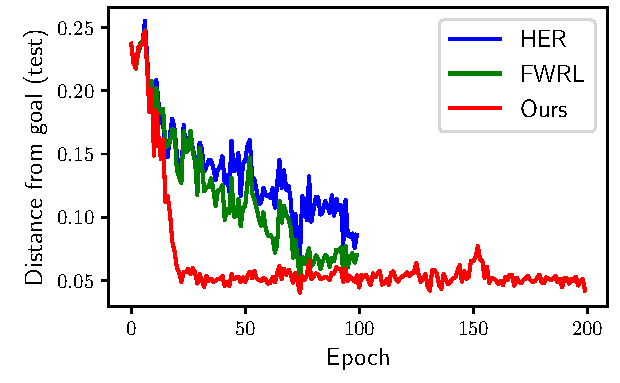
\includegraphics[width=\frac\columnwidth]{media/res/6efc1de-path_reward_low_thresh_chosen-FetchPickAndPlacePR-v1-dqst/epoch-test/ag_g_dist.pdf}
  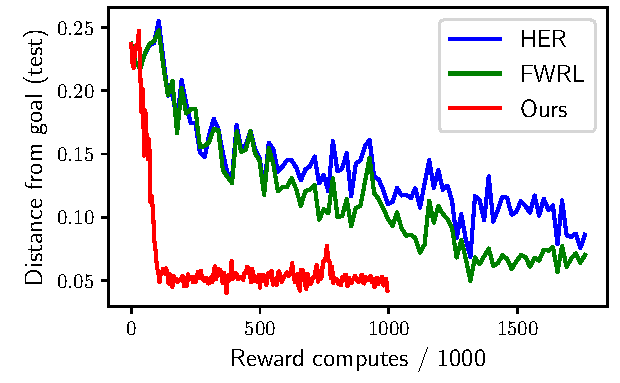
\includegraphics[width=\frac\columnwidth]{media/res/6efc1de-path_reward_low_thresh_chosen-FetchPickAndPlacePR-v1-dqst/reward_computes-test/ag_g_dist.pdf}%
  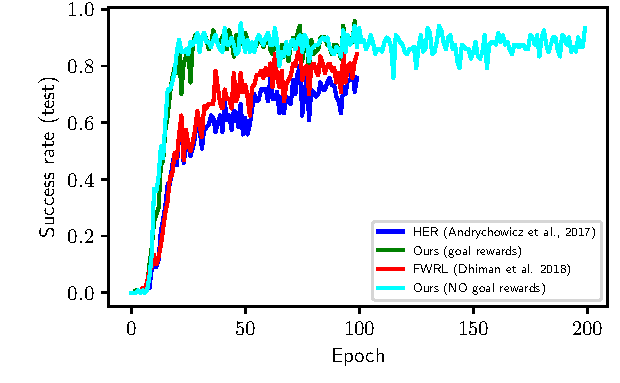
\includegraphics[width=\frac\columnwidth]{media/res/6efc1de-path_reward_low_thresh_chosen-FetchPickAndPlacePR-v1-dqst/epoch-test/success_rate.pdf}%
  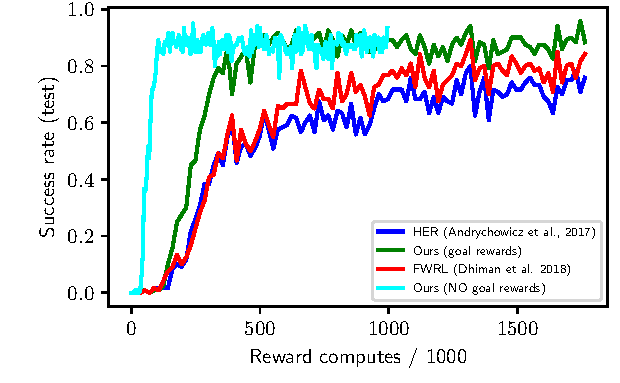
\includegraphics[width=\frac\columnwidth]{media/res/6efc1de-path_reward_low_thresh_chosen-FetchPickAndPlacePR-v1-dqst/reward_computes-test/success_rate.pdf}\\
  \rotatebox{90}{\tiny\hspace{2em}\color{blue}{Fetch Slide}}%
  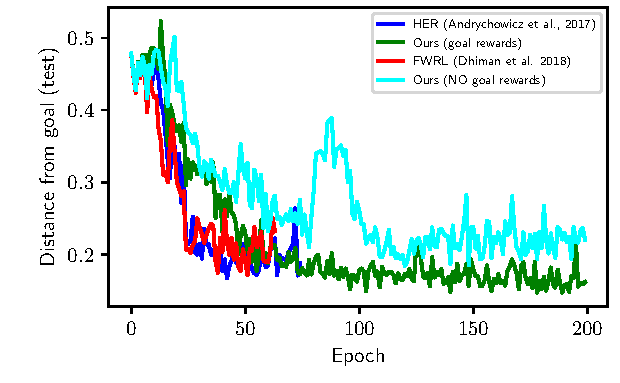
\includegraphics[width=\frac\columnwidth]{media/res/6efc1de-path_reward_low_thresh_chosen-FetchSlidePR-v1-dqst/epoch-test/ag_g_dist.pdf}
  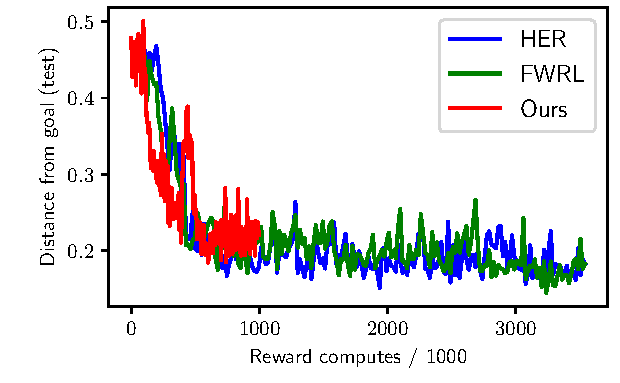
\includegraphics[width=\frac\columnwidth]{media/res/6efc1de-path_reward_low_thresh_chosen-FetchSlidePR-v1-dqst/reward_computes-test/ag_g_dist.pdf}%
  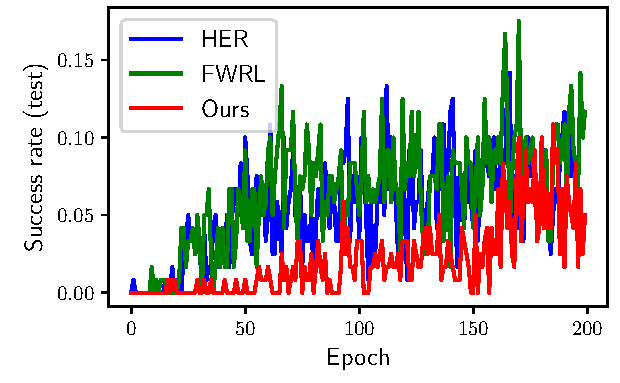
\includegraphics[width=\frac\columnwidth]{media/res/6efc1de-path_reward_low_thresh_chosen-FetchSlidePR-v1-dqst/epoch-test/success_rate.pdf}%
  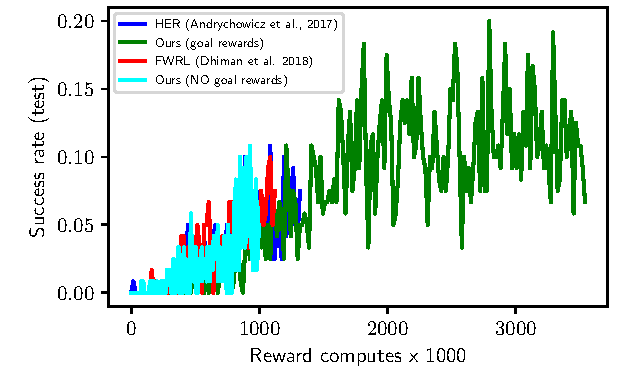
\includegraphics[width=\frac\columnwidth]{media/res/6efc1de-path_reward_low_thresh_chosen-FetchSlidePR-v1-dqst/reward_computes-test/success_rate.pdf}\\
  {.\tiny\color{blue}\hspace{0.8cm}(a) Distance on Epochs \hspace{1.05cm}(b) Distance on
    reward computes
    \hspace{0.70cm} (c) Success rate on epochs \hspace{0.9cm} (d) Success rate on reward computes}
  \label{fig:path-reward-fetch}%
  \caption{We compare our method against HER~\citep{andrychowicz2016learning}
    and FWRL~\citep{dhiman2018floydwarshall}.
For Fetch Reach and Push tasks our method achieves comparable performance
across both metrics, the success rate and the distance to the goal. In the Fetch
%Pick and Place task, our method outperforms the baselines. However, for Fetch
%Slide task the opposite is true.
%When the number of reward computations is take into account our method learns
%much faster than across all tasks.
  }%
\end{figure}
